%!TEX root = slides.tex


% 1. Basics
% 2. Recursion (numbers/lists)
% 3. MapReduce

\section{Racket}

\begin{frame}{Alonzo Church}
  \begin{columns}
    \begin{column}{1.5in}
      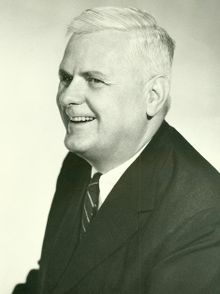
\includegraphics[width=1.4in]{img/church.jpg}
    \end{column}
    \begin{column}{0.7\textwidth}
      \begin{itemize}
        \item Alonzo Church (1903 -- 1995) supervised PhDs of Alan Turing, Stephen Kleene, John George Kemeny, and many others.
        \vspace{5mm}
        \item Introduced lambda calculus:
          $$ \lambda f . ( \lambda x . f ( x x ) ) ( \lambda . f ( x x ) )$$
        \item Church--Turing thesis: lambda calculus represents all possible computations (so do Turing machines).
      \end{itemize}
    \end{column}
  \end{columns}
  \citeurl{wikipedia.org/wiki/Alonzo\_Church}
\end{frame}

\begin{frame}{John McCarthy}
  \begin{columns}
    \begin{column}{1.5in}
      \includegraphics[width=1.4in]{img/john-mccarthy.png}
    \end{column}
    \begin{column}{0.7\textwidth}
      \begin{itemize}
        \item John McCarthy developed LISP at MIT in the late 1950s.
        \vspace{1mm}
        \item Also famous for coining the term \emph{artificial intelligence} at the Dartmouth workshop in 1956.
        \vspace{1mm}
        \item Lisp generally considered first functional programming language: based on lambda calculus, limited side effects, first-class functions.
        \vspace{1mm}
        \item Lots of dialects exist today, such as Scheme, Racket and Common Lisp.
      \end{itemize}
    \end{column}
  \end{columns}
  \citeurl{www-formal.stanford.edu/jmc/}
\end{frame}

\begin{frame}[fragile]{Wasteful for loops}
  \begin{minted}{python}
# How do you parallelise this?
inds = list(range(10))
total = 0
for i in inds:
  total = total + (i * 7)
  \end{minted}
  \begin{minted}{python}
def byseven(i):
  return i * 7

inds = list(range(10))
sevens = map(byseven, inds)
total = sum(sevens)
  \end{minted}
\end{frame}

\begin{frame}{State}
\begin{description}
  \item[Imperative] programming is a programming paradigm where statements are used to change the \emph{state}.
  \item[State] is the name given to the current data/values related to an executing process, including internal stuff like the call stack.
  \item[Processes] begin with an initial state and (possibly) have (a number of) halt states.
  \item[Statements] change the state.
  \item[Functions] in imperative programming languages might return different values for the same input at different times, because of the state.
  \item[Functional] programming languages (try to) not depend on state.
\end{description}
\end{frame}


\begin{frame}{Side effects}
  \begin{description}
    \item[Functions] are said to have side effects if they modify the state (on top of returning a value).
    \item[Static and global] variables are often good examples of side effects in action.
    \item[Functional] programming tries to avoid side effects.
    \item[It's tricky] to avoid them -- such as when we need user input.
  \end{description}
\end{frame}

\begin{frame}[fragile]{Basic operators}
\begin{minted}{scheme}
> (+ 3 4)
7
> (* 3 2)
6
> (- 5 3)
2
> (/ 6 3)
2
\end{minted}
\end{frame}

\begin{frame}[fragile]{More arguments}
\begin{minted}{scheme}
> (+ 3 4 5)
(+ 3 4 5)
> (- 3 4 5)
-6
> (* 2 3 4)
24
> (/ 6 3 3)
2/3
> (/ 6 3 3 3)
2/9
\end{minted}
\end{frame}


\begin{frame}[fragile]{Functions and values}
\begin{minted}{scheme}
; Define a value called foo with value 3.
>(define foo 3)

; Define a function f.  
>(define (f x)
  (+ (* 3 x) 12))

>(define (g x)
  (* 3 (+ x 4)))

>(g 2)
18
\end{minted}
\citeurl{www.artificialworlds.net/presentations/scheme-01-intro/scheme-01-intro.html}
\end{frame}

\begin{frame}[fragile]{Conditionals}
  \begin{minted}{scheme}
> (if (< 1 2) '(y e s) '(n o))
(y e s)

>(define (abs x)
  (if (< x 0)
  (- x)
  x))

\end{minted}
\citeurl{www.artificialworlds.net/presentations/scheme-01-intro/scheme-01-intro.html}
\end{frame}


\begin{frame}[fragile]{Lists}
  \begin{minted}{scheme}
>(list 1 2 3)
(1 2 3)

>(list 'a 'b 'c)
(a b c)

> (length (list 1 2 3))
3
\end{minted}
\citeurl{www.artificialworlds.net/presentations/scheme-01-intro/scheme-01-intro.html}
\end{frame}

\begin{frame}[fragile]{car and cdr}
  \begin{minted}{scheme}
> (car (list 1 2 3))
1
> (cdr (list 1 2 3))
(2 3)
> (define l (list 1 2 3))
> (car l)
1
> (cdr l)
(2 3)
> (car (cdr l))
2
> (cadr l)
2
\end{minted}
\citeurl{www.artificialworlds.net/presentations/scheme-01-intro/scheme-01-intro.html}
\end{frame}

\begin{frame}[fragile]{Recursion}
  \begin{minted}{scheme}
> (define (sum lv)              
    (if (null? lv)
      0
      (+ (car lv) (sum (cdr lv)))))
> (sum (list 1 2 3))                            
6
> (define (derange n)
    (if (= 0 n)
      '()
      (cons n (derange (- n 1)))))
> (derange 12)                                                    
(12 11 10 9 8 7 6 5 4 3 2 1)
\end{minted}
\citeurl{www.artificialworlds.net/presentations/scheme-01-intro/scheme-01-intro.html}
\end{frame}

\begin{frame}[fragile]{Looping recursively}
\begin{minted}{scheme}
> (let loop ((i 5))
(print "i is " i ".\n")
(if (> i 0) (loop (- i 1))))
i is 5.
i is 4.
i is 3.
i is 2.
i is 1.
i is 0.
\end{minted}
\citeurl{gambitscheme.org/wiki/images/a/a7/A\_Tour\_of\_Scheme\_in\_Gambit.pdf}
\end{frame}

\begin{frame}[fragile]{Data and code}
\begin{minted}{scheme}
> (define (swap3-1-2 x)
  (list (cadr x) (car x) (caddr x)))

> (swap3-1-2 (list 1 2 3))
(2 1 3)

> (define four-over-two (list 4 '/ 2))

> four-over-two
(4 / 2)

> (eval (swap3-1-2 four-over-two))
\end{minted}
\citeurl{www.artificialworlds.net/presentations/scheme-01-intro/scheme-01-intro.html}
\end{frame}

\begin{frame}[fragile]{More on functions}
\begin{minted}{scheme}
; Printing stuff to terminal.
> (print "Ay" "-" "yo.\n")
; Proper way to define a function.
> (define foo (lambda (bar) (print "Bar is " bar ".\n")))
; Shorthand.
> (define (foo bar) (print "Bar is " bar ".\n"))

; Local variables.
> (define (foo bar) (let ((thing "Bar"))
    (print thing " is " bar ".\n")))
> (foo "open")
Bar is open.
\end{minted}
\citeurl{gambitscheme.org/wiki/images/a/a7/A\_Tour\_of\_Scheme\_in\_Gambit.pdf}
\end{frame}

\begin{frame}[fragile]{Function example}
  \begin{minted}{scheme}
> (define l 
    (let
      ((d 4) (e 5))
      (lambda (a b c) (list a b c d e))
    )
  )
> (l 1 2 3)
(1 2 3 4 5)
  \end{minted}
  \citeurl{gambitscheme.org/wiki/images/a/a7/A\_Tour\_of\_Scheme\_in\_Gambit.pdf}
\end{frame}

\begin{frame}[fragile]{cons}
\begin{minted}{scheme}
> (cons 1 '())
(1)
> (cons 1 (cons 2 null))
(1 2)
> (cons 1 (cons 2 (cons 3 null)))
(1 2 3)
> (define mylist (cons 1 (cons 2 (cons 3 null))))
> mylist
(1 2 3)
> (car mylist)
1
> (cdr mylist)
(2 3)
\end{minted}
\citeurl{www.artificialworlds.net/presentations/scheme-02-basics/scheme-02-basics.html}
\end{frame}

\begin{frame}[fragile]{More on lists}
\begin{minted}{scheme}
> (list "a" "b" "c")
("a" "b" "c")
> (list a b c)
reference to undefined identifier: a
> (list 'a 'b 'c)
(a b c)

> (equal? 
(list 1 2 3)
(cons 1 (cons 2 (cons 3 '()))))
#t
\end{minted}
\citeurl{www.artificialworlds.net/presentations/scheme-02-basics/scheme-02-basics.html}
\end{frame}

\begin{frame}[fragile]{Quoting}
\begin{minted}{scheme}
> (list a b c)
*** ERROR IN (console)@1.7--Unbound variable: a
> (quote (a b c))
(a b c)
> (quote a b c)
*** ERROR IN (console)@2.1--Ill-formed special form: quote
> '(a b c) 
(a b c)
> (define forty-two '(* 6 9))
> forty-two
(* 6 9)
> (eval forty-two)
54
\end{minted}
\citeurl{www.artificialworlds.net/presentations/scheme-05-quotation/scheme-05-quotation.html}
\end{frame}

\begin{frame}[fragile]{Null list}
\begin{minted}{scheme}
> ()
missing procedure expression
> (list)
()
> '()
()
> null
()
> 'null
null
\end{minted}
\citeurl{www.artificialworlds.net/presentations/scheme-05-quotation/scheme-05-quotation.html}
\end{frame}

\begin{frame}[fragile]{Closures}
\begin{minted}{scheme}
> (define (container value)
(lambda ()
(string-append "This container contains " value ".")))
> (define apple (container "an apple"))
> (define pie (container "a pie"))
> (apple)
"This container contains an apple."
> (apple)
"This container contains an apple."
> (pie)
"This container contains a pie."
\end{minted}
\citeurl{gambitscheme.org/wiki/images/a/a7/A\_Tour\_of\_Scheme\_in\_Gambit.pdf}
\end{frame}
